% TODO: 
%
% (1) GenRelObs and propagate fixes to text
%- i's where they shouldn't be, 
%- integrating over discrete vars, 
%- P(z_k|...) needs to condition on belief state, 
%- line 13 generates does not get rid of xd_s'... did you mean to integrate out alpha(xd_o,xd_s) instead?
% ... \delta_j(x_{d_o}) should integrate out to 1 right?
%     then use this?
%
% (2) Notation for observation set
%
% (3) Improve intuitions
%
% (4) Revise conclusion
%
% (5) More formal claims, where this works, where PBVI exact

\documentclass{article} % For LaTeX2e
\usepackage{nips12submit_e,times}
%\documentstyle[nips12submit_09,times,art10]{article} % For LaTeX 2.09

\def\argmax{\operatornamewithlimits{arg\max}}

\title{Symbolic Dynamic Programming for Continuous State and Observation POMDPs}


\author{
%Zahra Zamani \\
%ANU & NICTA\\
%Canberra, Australia \\
%\texttt{zahra.zamani@anu.edu.au} \\
%\And
%Coauthor \\
%Affiliation \\
%Address \\
%\texttt{email} \\
%\AND
%Coauthor \\
%Affiliation \\
%Address \\
%\texttt{email} \\
%\And
%Coauthor \\
%Affiliation \\
%Address \\
%\texttt{email} \\
%\And
%Coauthor \\
%Affiliation \\
%Address \\
%\texttt{email} \\
%(if needed)\\
}

% The \author macro works with any number of authors. There are two commands
% used to separate the names and addresses of multiple authors: \And and \AND.
%
% Using \And between authors leaves it to \LaTeX{} to determine where to break
% the lines. Using \AND forces a linebreak at that point. So, if \LaTeX{}
% puts 3 of 4 authors names on the first line, and the last on the second
% line, try using \AND instead of \And before the third author name.

\newcommand{\open}{\mathit{open}}
\newcommand{\close}{\mathit{close}}
\newcommand{\high}{\mathit{high}}
\newcommand{\low}{\mathit{low}}
\newcommand{\fix}{\marginpar{FIX}}
\newcommand{\new}{\marginpar{NEW}}

%\nipsfinalcopy % Uncomment for camera-ready version

\begin{document}

\maketitle

\begin{abstract}
Partially-observable Markov decision processes (POMDPs) provide a
powerful model for real-world sequential decision-making problems.  In
recent years, point-based value iteration methods have proven to be
extremely effective techniques for finding (approximately) optimal
dynamic programming solutions to POMDPs when an initial set of belief
states is known.  However, no point-based work has provided exact
point-based backups for both continuous state and observation spaces,
which we tackle in this paper.  Our key insight is that while there
may be an infinite number of possible observations, there are only a
finite number of observation partitionings that are relevant for
optimal decision-making when a finite, fixed set of reachable belief
states is known.  To this end, we make two important contributions:
(1) we show how previous exact symbolic dynamic programming solutions
for continuous state MDPs can be generalized to continuous state
POMDPs with discrete observations, and (2) we show how this solution
can be further extended via recently developed symbolic methods to
continuous state and observations to \emph{derive} the minimal
relevant observation partitioning for potentially correlated,
multivariate observation spaces.
%for domais with piecewise
%polynomial transition and observation functions.  
We demonstrate our algorithm on a power plant
control problem requiring continuous state 
\emph{and} observations.
%empirically evaluate on real-world inspired power 
%proof-of-concept results on uni- and multi-variate state and
%observation power plant control.
\end{abstract}

\section{Introduction} %and Related Work}
% Write intro here

Partially-observable Markov decision processes (POMDPs) are a powerful
modeling formalism for real-world sequential decision-making
problems~\cite{kaebling}.  In recent years, point-based value
iteration methods~\cite{pbvi_jair06,hsvi2,Perseus,gapmin} have proved
extremely successful at scaling (approximately) optimal POMDP
solutions to large state spaces when a set of initial belief states is
known.

More recent work has extended point-based methods to both continuous
state and continuous observation spaces, but no work has tackled both
jointly without sampling.  \cite{Perseus_cont} provides exact
point-based backups for continuous state and discrete observation
problems (with approximate sample-based extensions to continuous
actions and observations), while~\cite{pascal_ijcai05} provides exact
point-based backups for discrete state and continuous observation
problems (where multivariate observations must be conditionally
independent).  While
restricted to discrete states, \cite{pascal_ijcai05} provides an
important insight that we exploit in this work: \emph{only a finite
number of partitionings of the observation space are required to
distinguish between the optimal conditional policy over a finite set
of belief states}.

Our contributions in this work are two-fold.  First, we extend
symbolic dynamic programming for continuous state
MDPs~\cite{sanner_uai11} to the case of continuous state and discrete
observation POMDPs.  This provides an expressive and concrete
instantiation of the framework in~\cite{Perseus_cont} (which only
abstractly required that integrals were computable) in that it ensures
the closed-form of all $\alpha$-functions for \emph{all horizons} is a
symbolic piecewise case statement, even for POMDPs with
\emph{arbitrary} continuous rewards and transitions with discrete
noise (i.e., a finite mixture of deterministic transitions).  
Second, we extend this symbolic dynamic programming algorithm
to the case of continuous observations (while restricting the
transition to piecewise linear functions and the reward functions to piecewise constants) and extend
the work of~\cite{pascal_ijcai05} to \emph{derive} relevant observation
partitions for potentially correlated multivariate continuous
observation spaces by exploiting the piecewise polynomial integration
operation of~\cite{sanner_aaai12} and the multivariate symbolic maximization
technique of~\cite{sanner_uai11}.  
We conclude by demonstrating our algorithm on a power plant
control problem requiring bivariate continuous state and observations.

%\footnote{All code for these
%experiments is freely available online (link suppressed) and
%attached as anonymized supplementary material to this submission.}

%We proceed as follows: after reviewing POMDPs, we discuss the need for 
%first-order POMDPs, formalize them, and provide a lifted solution
%via symbolic dynamic programming (SDP).  We empirically show the
%complexity of SDP is invariant to domain size while enumerated
%state POMDP solvers have complexity exponential in the domain size.

\section{DC-POMDP Model} 

We assume familiarity with MDPs and introduce discrete and continuous
partially observable MDPs (DC-POMDPs) as an extension to their DC-MDP
subset~\cite{sanner_uai11}.  A DC-POMDP is a tuple $\langle
\mathcal{S},\mathcal{A},\mathcal{O},\mathcal{T},\mathcal{R},\mathcal{Z},\gamma,h
\rangle$.  States $\mathcal{S}$ are represented by vectors of
$(\vec{d_s},\vec{x_s}) = (
d_{s_1},\ldots,d_{s_n},x_{s_1},\ldots,x_{s_m} )$ where each $d_{s_i}
\in \{ 0,1 \}$ ($1 \leq i \leq n$) is a discrete boolean and each
$x_{s_j} \in \mathbb{R}$ ($1 \leq j \leq m$) is a continuous variable.
We assume a finite, discrete action space $\mathcal{A} = \{ a_1,
\ldots, a_p \}$. Observations
$\mathcal{O}$ are given by the vector $(\vec{d_o},\vec{x_o}) = (
d_{o_1},\ldots,d_{o_p},x_{o_1},\ldots,x_{o_q} )$ where each $d_{o_i}
\in \{ 0,1 \}$ ($1 \leq i \leq p$) is boolean and each $x_{o_j} \in
\mathbb{R}$ ($1 \leq j \leq q$) is continuous.

Three functions are required for modeling DC-POMDPs: (1) $\mathcal{T}: \mathcal{S} \times \mathcal{A} \times \mathcal{S} \rightarrow  [ 0, 1 ]$ a Markovian transition model defined as the probability of the next state given the action and previous state%$P(\vec{d}',\vec{x}'|\cdots,a)$
; (2)  $\mathcal{R}:\mathcal{S}\times\mathcal{A} \rightarrow \mathbb{R}$ a reward function which returns the immediate reward of taking an action in some state; and (3) an observation function defined as $\mathcal{Z} : \mathcal{S} \times \mathcal{A} \times \mathcal{O} \rightarrow [ 0, 1 ]$  which gives the probability of an observation given the outcome of a state after executing an action.  A discount factor $\gamma, \; 0 \leq \gamma \leq 1$ is used to discount rewards $t$ time steps into the future by $\gamma^t$.

We use a dynamic Bayesian network (DBN) to compactly represent the transition model over the factored state variables and we likewise use a Bayesian network to represent the observation model:
{\footnotesize
\begin{align*}
\mathcal{T}: \;\; &
P(\vec{d_s}',\vec{x_s}'|\vec{d_s},\vec{x_s},a) = 
\prod_{i=1}^n P(d_{s_i}'|\vec{d_s},\vec{x_s},a) \prod_{j=1}^m P(x_{s_j}'|\vec{d_s},\vec{d_s}',\vec{x_s},a). \nonumber \\
\mathcal{Z}: \;\; & 
P(\vec{d_o},\vec{x_o}|\vec{d_s},\vec{x_s},a) = 
\prod_{i=1}^n P(d_{o_i}|d_{s_i},a) \prod_{j=1}^m P(x_{o_j}|x_{s_j},a). \nonumber 
\end{align*}}
For simplicity of algorithmic exposition, we do not allow synchronic
arcs in the transition representation, but note that to incorporate
such arcs only requires restrictions on the variable elimination
ordering during dynamic programming.  In these transition and
observation Bayes nets, 
probabilities over 
\emph{discrete} variables are represented using conditional probability
functions (CPF) in the form of
$P(d_i'|\vec{d},\vec{x},a)$. Probabilities for \emph{continuous} variables
$P(x_j'|\vec{d},\vec{d'},\vec{x},a)$ are represented by
\emph{piecewise linear functions} (PLFs) that are first-order Markov
and deterministic, i.e. the probabilities are encoded using the Dirac
$\delta[\cdot]$ function. The reward function $R(\vec{d},\vec{x},a)$
is set to a piecewise constant function. We next provide an intuitive
example to make this DC-POMDP framework more concrete.
%%%%%%%%%%%%%%%%%%%%%%%%%%%%%%%%%%%%%%%%%%%%%%%%%%%%%%%%%%%%%%%%%%%%%%%%
% Figure 1 - policy tree
\begin{figure}[t!]
%\vspace{-1mm}
\begin{center}
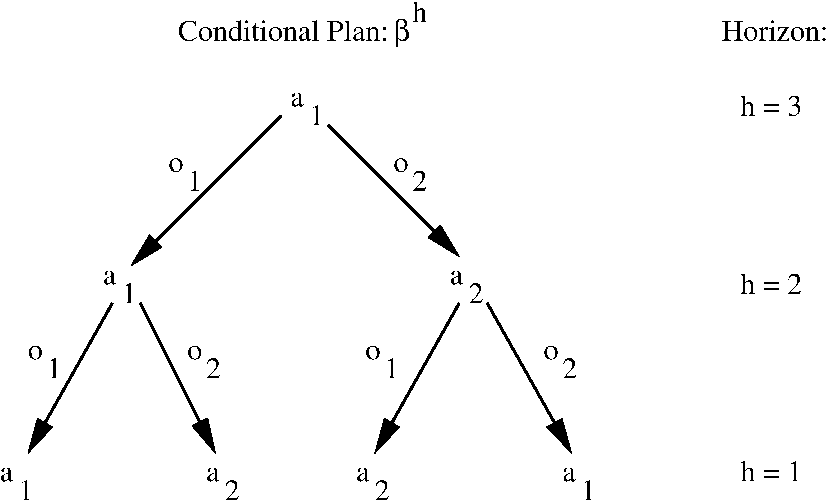
\includegraphics[width=0.4\textwidth]{pics/cond_plan2.pdf}
\hspace{5mm}
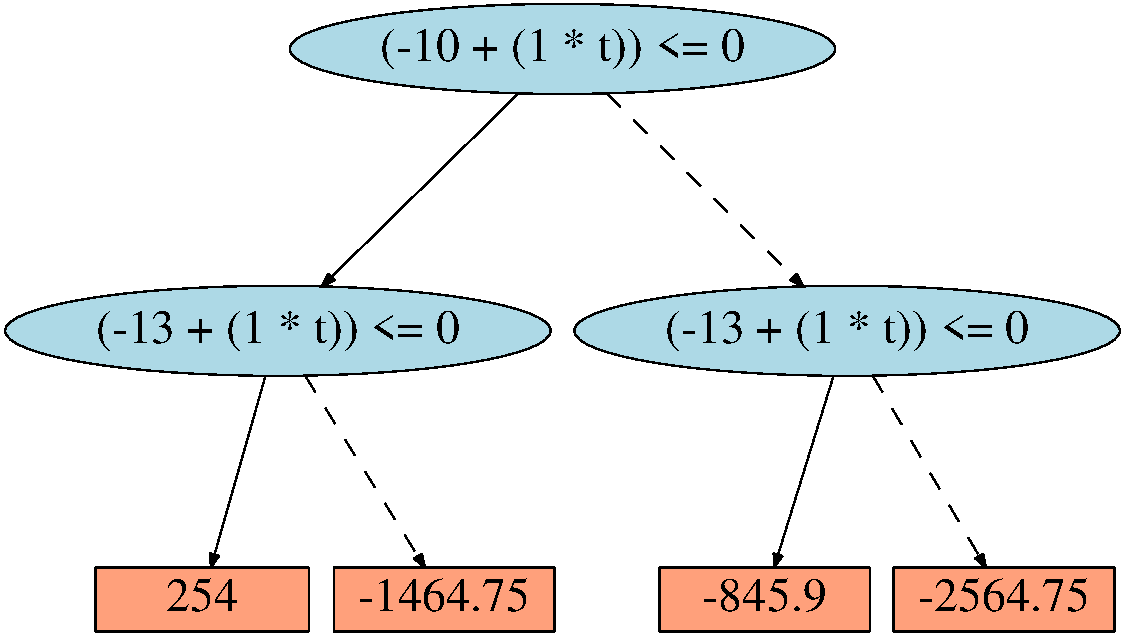
\includegraphics[width=0.45\textwidth]{pics/b1-4.pdf}
\end{center}
\vspace{-2mm}
\caption{\footnotesize (left) Example conditional plan $\beta^h$ for discrete observations; (right) an example piecewise $\alpha$-vector for continuous state $t$ represented
as a 
%The maximum $\alpha$ vector for a belief state at iteration 4 for the \textsc{\bf Power Plant} problem in Section~\ref{}
decision diagram: 
the \emph{true} branch is solid, the \emph{false}
branch is dashed.}
\label{fig:cond_plan}
\vspace{-1mm}
\end{figure}
%%%%%%%%%%%%%%%%%%%%%%%%%%%%%%%%%%%%%%%%%%%%%%%%%%%%%%%%%%%%%%%%%%%%%%%%
%%%%%%%%%%%%%%%%%%%%%%%%%%%%%%%%%%%%%%%%%%%%%%%%%%%%%%%%%%%%%%%%%%%%%%%%%%%
%\begin{figure}[t]
%\begin{center}
%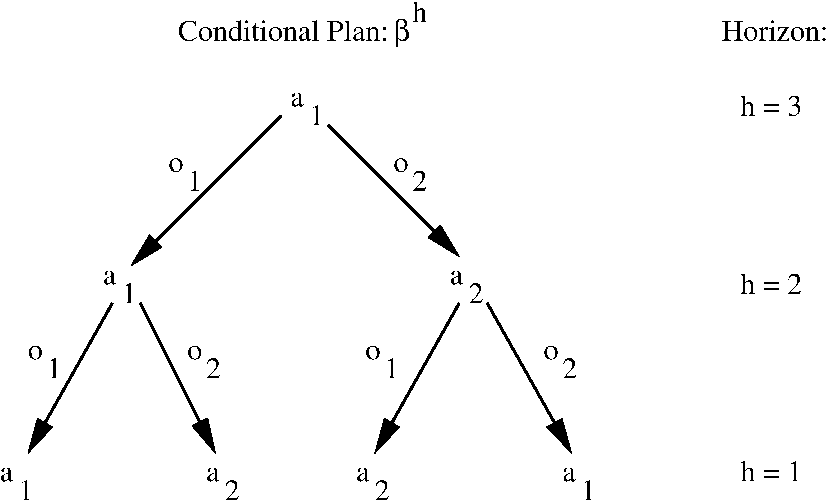
\includegraphics[width=0.4\textwidth]{pics/cond_plan2.pdf}
%\end{center}
%\vspace{-3mm}
%\caption{%\footnotesize 
%The optimal value function for \textsc{\bf Power Plant}
%as a decision diagram: 
%the \emph{true} branch is solid, the \emph{false}
%branch is dashed.} 
%\end{figure}
%%%%%%%%%%%%%%%%%%%%%%%%%%%%%%%%%%%%%%%%%%%%%%%%%%%%%%%%%%%%%%%%%%%%%%%%%%%

\textbf{Example} \textsc{\bf (Power Plant)~\cite{steam2}} \emph{The steam
generation system of a power plant aims to provide hot steam to the
steam turbine which in turn produces electricity. Feed-water is
exposed to heat in the tubes leading to the water tank, where water
evaporation is performed under specific pressure and temperature.
A reward is obtained when electricity is generated through steam
production and the pressure and temperature are within safe ranges.
Mixing water and steam makes the
respective pressure and temperature observations $p_o \in \mathbb{R}$
and $t_o \in \mathbb{R}$ on the underlying state $p_s \in \mathbb{R}$
and $t_s \in \mathbb{R}$ highly uncertain.  Action choices are either
to open or close a pressure valve $a \in \{ \open, \close \}$.}

We initially present two 
simple examples labeled \textsc{\bf 1D-Power Plant} 
using only the temperature state $t_s$.
First, the transition and reward functions common to both problems
are defined as below where simply, the temperate increments or
decrements according to the action:
% For the transition probability, we use the Dirac function to model the deterministic equations. We can also define stochasticity in the transition model using boolean random variables that are sampled stochastically.  The reward function can be any linear function of the state or action. Going above a threshold temperature (e.g. $T=10$) will cause an explosion in the plant when trying to close the valve which results in the negative reward of $-1000$. Staying below this temperature is safe and will produce electricity an gain the reward of $100$. The reward of an open valve is $-1$.
{\footnotesize
\vspace{-1mm}
\begin{align}
\label{eq:trans}
P(t_s'|\vec{t_s},a)= \delta\left[ t_s' - 
\begin{cases}
 (a=\open) &: t_s - 5 \\ 
(a \neq \open) &: t_s + 7 \\
\end{cases}
\right]
\hspace{2mm}
R(t_s,a) = 
\begin{cases}
 (a=\open) &: -1 \\
(a \neq \open)\wedge (t_s>T) &: -1000 \\
(a \neq \open)\wedge \neg(t_s>T) &: 100 \\
\end{cases}
\end{align}
\vspace{-4mm}
}

%contribution? 
Next we introduce the \textsc{\bf Discrete Obs. 1D-Power Plant} variant using 
a discrete binary observation space with possible
observations $o \in \mathcal{O} = \{\high,\low\}$:
{\footnotesize
\vspace{-1mm}
\begin{align}
P(o=\high|t_s',\open) = 
\begin{cases}
  t_s' <= 15 &: 0.9 \\
 \neg (t_s' <= 15)&: 0.1 \\
\end{cases}
\hspace{5mm}
P(o=\low|t_s',\open) = 
\begin{cases}
 t_s' <= 15 &: 0.1 \\
 \neg (t_s' <= 15) &: 0.9 \\
\end{cases}
\end{align}
\vspace{-3mm}
}
%\\
%P(t_{o_1}|t_s',\close) = 
%\begin{cases}
% \delta\left[ t_s <= 15 \right] &: 0.1 \\
% \delta\left[ \neg (t_s <= 15)\right] &: 0.8 \\
%\end{cases}\nonumber
%,
%P(t_{o_2}|t_s',\close) = 
%\begin{cases}
% \delta\left[ t_s <= 15 \right] &: 0.9 \\
% \delta\left[ \neg (t_s <= 15)\right] &: 0.2 \\
%\end{cases} \nonumber
%\end{align}

Finally we introduce the \textsc{\bf Cont. Obs. 1D-Power Plant}
variant with continuous observation $t_o$.  
We define the observation probability over $t_o$ as uniform on
an interval 10 units wide, centered at $t_s'$.
{\footnotesize
\begin{align}
P(t_o|t_s',\open) = 
\begin{cases}
 (t_o>t_s'-5) \wedge (t_o<t_s'+5) &: 0.1 \\
 \neg((t_o>t_s'-5) \wedge (t_o<t_s'+5)) &: 0 \\
\end{cases}
\end{align}
}
While the restrictions may seem too tight in our problems due to the continuous nature of the state and observation space, there has been no exact solution to any of the two set of problems above. 
\section{DC-POMDP solution}

In a DC-POMDP, the agent does not directly observe the states and thus
must maintain a belief state $b(xd_s) = P(xd_s)$.\footnote{For
compactness we define $xd_s := (x_s,d_s)$ and $xd_o:=(x_o,d_o)$.}  For a
given belief state $\vec{b} = b(\cdot)$, a POMDP policy $\pi$ can be
represented by a tree corresponding to a conditional plan $\beta$.  An
h-step conditional plan $\beta^h$ can be defined recursively in terms
of $(h-1)$-step conditional plans as shown in
Fig.~\ref{fig:cond_plan}.

Our goal is to find a policy $\pi$ that maximizes the value function,
defined as the sum of expected discounted rewards over horizon $h$
starting from initial belief state $\vec{b}$:
\begin{equation}
V^h_\pi(\vec{b}) = E_{\pi} \left[ \sum\nolimits_{t=0}^{h} \gamma^t \cdot r_t \Big| \vec{b}_0 = \vec{b} \right]
\end{equation}
where $r_t$ is the reward obtained at time $t$ and $\vec{b}_0$ is the
belief state at $t=0$.  For finite $h$ and belief state $\vec{b}$, the
optimal policy $\pi$ takes the form of an $h$-step conditional plan
$\beta^h$.  For $h = \infty$, the optimal discounted ($\gamma < 1$)
value function can be approximated arbitrarily closely by using
a sufficiently large, but finite $h$~\cite{kaebling}.  

Even when the state is continuous (but the actions and observations
are discrete), 
the optimal POMDP value function for finite horizon $h$ is a piecewise linear
and convex function of the belief state $\vec{b}$~\cite{Perseus_cont} hence 
$V^h$ is given by a maximum over a finite set of
``$\alpha$-vectors'' $\alpha^h_i$:
\begin{equation}
V^h(\vec{b}) = \max\nolimits_{\alpha^h_i \in \Gamma^h} \alpha^h_i \cdot \vec{b}
\end{equation}
Later on when we tackle continuous state \emph{and} observations,
we note that we will dynamically derive an optimal, 
finite partitioning of the observation
space for a given belief state and hence reduce the continuous
observation problem back to a discrete observation problem at every
horizon.  

The $\Gamma^h$ in this optimal $h$-stage-to-go value function can be
computed via Monahan's dynamic programming approach to \emph{value
iteration} (VI)~\cite{monahan82}.  
Initializing  $\alpha^0_1 = \vec{0}$ and $\Gamma^0 = \{ \alpha^0_1 \}$, $\Gamma^h$ is obtained from $\Gamma^{h-1}$ using the backup operation defined in (2) and considering $r_a = r(x_s,d_s,a)$ :\footnote{The $\textrm{\large $\boxplus$}$ of sets is defined as 
$\textrm{\large $\boxplus$}_{j \in \{ 1,\ldots, n \} } S_j = S_1 \textrm{\large $\boxplus$} \cdots \textrm{\large $\boxplus$} S_n$ where the pairwise cross-sum $P 
\textrm{\large $\boxplus$} Q = \{ \vec{p} + \vec{q} | \vec{p} \in P, \vec{q} \in Q \}$.}
{\footnotesize
\begin{align} 
g^h_{a,o,j} &=  \int_{x_{s'}} \sum_{d_{s'}} p(o|xd'_s,a)p(xd'_s|xd_s,a) \alpha^{h-1}_j(xd'_s) ; \hspace{2mm}  \forall \alpha^{h-1}_{j} \in \Gamma^{h-1} \label{eq:backup} \\
\Gamma^{h}_a   &= r_a + \gamma \textrm{\large $\boxplus$}_{o \in \mathcal{O}} \left\{ g^h_{a,o,j}(\cdot) \right\}_j  \label{eq:cross_prod}\\ 
\Gamma^h  &= \bigcup_a \Gamma^h_a 
\end{align}
}
\vspace{-3mm}
%%%%%%%%%%%%%%%%%%%%%%%%%%%%%%%%%%%%%%%%%%%%%%%%%%%%%%%%%%%%%%%%%%%%%%%%
\incmargin{.5em}
\linesnumbered
\begin{algorithm}[t!]
\vspace{-.5mm}
\dontprintsemicolon
\SetKwFunction{backup}{Backup}
\SetKwFunction{genObs}{GenRelObs}
\SetKwFunction{prune}{Prune}
\SetKwFunction{remapWithPrimes}{Prime}
\Begin
{
   $V^0:=0, h:=0, \Gamma_{PBVI}^0 = \{ \alpha_1^0 \} $\;
   \While{$h < H$}
   {
       $h:=h+1, \Gamma^h :=\emptyset, \Gamma_{PBVI}^h :=\emptyset$\;
       \ForEach {$b_i \in B$}
       {
       	\ForEach {$a \in A$}
      	 {
			$\Gamma_{a}^h :=\emptyset$ \;       		
       		\If {$ContObs =true$}
       			{\emph{// Continuous observation so derive observation set $O_i^h$ for belief $b_i$} \;
			  $(O_i^h,P(O_i^h|xd_{s})) \,:=\,$ \genObs{$\Gamma_{PBVI}^{h-1},a,b_i$}\;}
       		 \ForEach {$o \in \mathcal{O}_i^{h}$}
       		 {
				\ForEach {$\alpha_j^{h-1} \in \Gamma_{PBVI}^{h-1}$}
       			{
   	 		  		$\alpha_j^{h'-1},:=\,$ \remapWithPrimes{$\alpha_j^{h-1}$} 
   	 		  		\emph{// $\forall$ $d_i \to d_i'$ and $\forall x_i \to x_i'$} \; 
%   	 		    	$\Gamma_{a,xd_{o_i},j}^h \,:=\, P(o|xd_{s}) \cdot$ \backup{$\alpha_j^{h'},a$}\;
   	 		    	{$g_{a,o,j}^h \,:=\, $ see Eq~\eqref{eq:backup}}
       	      	}
%       	      	$\Gamma_{a,xd_o}^h\,:=\,\textrm{\large $\boxplus$} \Gamma_{a,xd_{o_i}}^h$\;
%       	      	$\Gamma_{a,xd_o}^h\,:=\, $ see Eq~\eqref{eq:cross_prod}\;
       	     }
%           $\Gamma_a^{h} \,:=\,R_a \oplus \gamma \cdot \Gamma_{a,xd_o}^h$\;
            $\Gamma_a^{h} \,:=\, $ see Eq~\eqref{eq:cross_prod}\;
            $\Gamma^{h} \,:=\, \Gamma^{h} \cup \Gamma_a^{h}$\;
       	 }  
        	%monahan's pruning first generates all vectors, then prunes
              $\Gamma^h \,:=\, $\prune{$\Gamma^h$} \emph{//optional step}\; 
      }
             % $V^h \,:=\, \mathrm{max}_{\alpha_j \in \Gamma^h} b_i \cdot \alpha_j$\;
             % $\pi^{*,h} \,:=\, \argmax_{a} \, \Gamma_a^{h}$\;
      \ForEach {$b_i \in B$}
      {
     	$\alpha_{b_i}^h :=\ \argmax_{\alpha_j \in \Gamma^h} \alpha_j \cdot b_i$\;
     	$\Gamma_{PBVI}^h :=\ \Gamma_{PBVI}^h \cup \alpha_{b_i}^h$\;
      }

       \If{$\Gamma_{PBVI}^h = \Gamma_{PBVI}^{h-1}$}
           {break $\,$ \emph{// Terminate if early convergence}\;}
   }
     \Return{$\Gamma_{PBVI}$} \;
}
\caption{\footnotesize \texttt{PBVI}(DC-POMDP, $H$,$ContObs$, $B=\left\{b_i \right\}$) $\longrightarrow$ $(V^h,\pi^{*,h})$ \label{alg:vi}}
\vspace{-1mm}
\end{algorithm}
\decmargin{.5em}
%%%%%%%%%%%%%%%%%%%%%%%%%%%%%%%%%%%%%%%%%%%%%%%%%%%%%%%%%%%%%%%%%

\textbf{Point-based value iteration (PBVI)} computes the optimal value function only for a set of belief states $\{ b_i \}$ where $b_i := P(xd_s)$.  The idea is straightforward and the main modification needed to Monahan's algorithm in Algorithm~\ref{alg:vi} is the loop from lines 19--21 where only $\alpha$-vectors optimal at some belief state are retained for subsequent iterations.  We note that \emph{if} all beliefs reachable in $h$ steps from some initial set can be finitely enumerated and PBVI is executed for this set of beliefs, then optimality is guaranteed for the PBVI policy over these initial beliefs up to horizon $h$.  
%In actuality in the DC-POMDP setting, the generation of continuous observations will most often lead to an infinite number of reachable belief states even in one step, so this optimality guarantee of PBVI will only hold for DC-POMDPs in very special cases when the set of reachable beliefs is finite.  Nonetheless, PBVI has been quite successful in practice without exhaustive enumeration of all reachable beliefs~\cite{pbvi_jair06,hsvi2,Perseus,gapmin}, which motivates our use of PBVI in this work.

We pause for a moment to make a few notes about the \texttt{PBVI}
algorithm in the context of DC-POMDPs.  If we have a fixed discrete
observation set, i.e., $\forall h \, \mathcal{O}^h = \mathcal{O}$, then
the algorithm proceeds as usual, but if we have continuous observation
variables then we will need to derive a relevant set of observations
on line 10, which we describe in Section~\ref{sec:cont_obs}.  We need
to guarantee that the integral on line 14 can be done in closed-form
and we guarantee this for the piecewise functions in
Section~\ref{sec:disc_obs}. We also note that the beliefs are piecewise constant functions. Because in general we will deal with
$\alpha$-functions represented as piecewise functions, we only assume
that strict dominance testing is implemented for \texttt{Prune} in
line 18.


\section{Symbolic Dynamic Programming} 

In this section we take a symbolic dynamic programming (SDP) approach
to performing \texttt{PBVI} in Algorithm~\ref{alg:vi}.  This requires
us to define all of the operations used in \texttt{PBVI} on a
closed-form representation.  For SDP, this closed-form will be a
piecewise case statement and it will be stored compactly as a decision
diagram~\cite{sanner_uai11}.  We first review this form and then
proceed to define SDP operations specific to the case of DC-POMDPs.

\subsection{Case Representation and Extended ADDs}
\label{sec:case}

% operations, max, restrict, substitute
%overview + example plant
The \textsc{\bf Power Plant} example represented all functions using
the case structure which can be generally defined as {\footnotesize
\vspace{-3mm}
\begin{align}
f = 
\begin{cases}
  \phi_1: & f_1 \\ 
 \vdots&\vdots\\ 
  \phi_k: & f_k \\ 
\end{cases} \nonumber
\end{align}
}
and this is the form we use to represent all functions in a DC-POMDP.
Here $\phi_i$ are disjoint logical formulae defined over the state $(\vec{d},\vec{x})$ with logical ($\land,\lor,\neg$) combinations of boolean variables and inequalities ($\geq,>,\leq,<$) over continuous variables.  
The $f_i$ are general functions, we will restrict them later for the
case of continuous observation POMDPs.

For \emph{unary operations} such as scalar multiplication $c\cdot f$ (for some constant $c \in \mathbb{R}$) or negation $-f$ on case statements is simply to apply the operation on each case partition $f_i$ ($1 \leq i \leq k$). 
A \emph{binary operation} on two case statements, takes the cross-product of the logical partitions of each case statement and performs the corresponding operation on the resulting paired partitions.  The cross-sum $\oplus$ of two cases is defined as the following:
{\footnotesize 
\vspace{-3mm}
\begin{center}
\begin{tabular}{r c c c l}
&
\hspace{-6mm} 
  $\begin{cases}
    \phi_1: & f_1 \\ 
    \phi_2: & f_2 \\ 
  \end{cases}$
$\oplus$
&
\hspace{-4mm}
  $\begin{cases}
    \psi_1: & g_1 \\ 
    \psi_2: & g_2 \\ 
  \end{cases}$
&
\hspace{-2mm} 
$ = $
&
\hspace{-2mm}
  $\begin{cases}
  \phi_1 \wedge \psi_1: & f_1 + g_1 \\ 
  \phi_1 \wedge \psi_2: & f_1 + g_2 \\ 
  \phi_2 \wedge \psi_1: & f_2 + g_1 \\ 
  \phi_2 \wedge \psi_2: & f_2 + g_2 \\ 
  \end{cases}$
\end{tabular}
\end{center}
\vspace{-2mm}
}
Likewise $\ominus$ and $\otimes$ are defined by subtracting or multiplying partition values.  Inconsistent partitions can be discarded when they are irrelevant to the function value.
A \emph{symbolic case maximization} is defined as below:
\vspace{-4mm}
{\footnotesize
\vspace{-2mm}
\begin{center}
\begin{tabular}{r c c c l}
&
\hspace{-7mm} $\mathrm{max} \Bigg(
  \begin{cases}
    \phi_1: \hspace{-2mm} & \hspace{-2mm} f_1 \\ 
    \phi_2: \hspace{-2mm} & \hspace{-2mm} f_2 \\ 
  \end{cases}$
$,$
&
\hspace{-4mm}
  $\begin{cases}
    \psi_1: \hspace{-2mm} & \hspace{-2mm} g_1 \\ 
    \psi_2: \hspace{-2mm} & \hspace{-2mm} g_2 \\ 
  \end{cases} \Bigg)$
&
\hspace{-4mm} 
$ = $
&
\hspace{-4mm}
  $\begin{cases}
  \phi_1 \wedge \psi_1 \wedge f_1 > g_1    : & \hspace{-2mm} f_1 \\ 
  \phi_1 \wedge \psi_1 \wedge f_1 \leq g_1 : & \hspace{-2mm} g_1 \\ 
  \phi_1 \wedge \psi_2 \wedge f_1 > g_2    : & \hspace{-2mm}f_1 \\ 
  \phi_1 \wedge \psi_2 \wedge f_1 \leq g_2 : & \hspace{-2mm} g_2 \\ 
  \vdots & \vdots
%  \phi_2 \wedge \psi_1 \wedge f_2 > g_1    : & \hspace{-2mm} f_2 \\ 
%  \phi_2 \wedge \psi_1 \wedge f_2 \leq g_1 : & \hspace{-2mm} g_1 \\ 
%  \phi_2 \wedge \psi_2 \wedge f_2 > g_2    : & \hspace{-2mm} f_2 \\ 
%  \phi_2 \wedge \psi_2 \wedge f_2 \leq g_2 : & \hspace{-2mm} g_2 \\ 
  \end{cases}$
\end{tabular}
\end{center}
\vspace{-3mm}
}
The following SDP operations on case statements require more detail than can be provided here, hence we refer the reader to the relevant literature:
\begin{itemize}
\item Restriction $f|_{\phi}$:  Takes a function $f$ to restrict only in cases
that satisfy some formula $\phi$ as defined in \cite{sanner_uai11}.
\item Substitution $f\sigma$ : Takes a set $\sigma$ of variables and their substitutions (which may be case statements), and carries out all variable substitutions in sequence~\cite{sanner_uai11}.
\item Integration $\int_{x_1} f dx_1$:  There are two forms: If $x_1$ is involved in a $\delta$-function (cf. the transition in Eq.~\eqref{eq:trans}) then the integral is equivalent to a symbolic substitution and can be applied to any case statement~\cite{sanner_uai11}. Otherwise, if $f$ is restricted to linear constraints and polynomial values, then the approach of~\cite{sanner_aaai12} can be applied to yield a result in the same form.
\end{itemize}
%\vspace{-2mm}
%\emph{Restriction} takes a function $f$ to restrict only in cases
%that satisfy some formula $\phi$, which we write as $f|_{\phi}$.  
%This can be done by simply appending $\phi$ to each case partition
%as the left side shows:
%{\footnotesize
%\begin{center}
%\begin{tabular}{r c c l}
%%&
%%\hspace{-6mm} 
%%  $f = \begin{cases}
%%    \phi_1: & f_1 \\ 
%%   \vdots&\vdots\\ 
%%    \phi_k: & f_k \\ 
%%  \end{cases}$
%%&
%&
%\hspace{0mm}
%  $f|_{\phi} = \begin{cases}
%    \phi_1 \land \phi : & f_1 \\ 
%   \vdots&\vdots\\ 
%    \phi_k \land \phi : & f_k \\ 
%  \end{cases}$
%&
%\hspace{15mm}
%$\int_{x_j'} P(x_j'|\cdots) V'^{h} dx_j' = \begin{cases}
%    \phi_1: & V'^{h} \{ x_j' = f_1 \} \\ 
%   \vdots&\vdots\\ 
%    \phi_k: & V'^{h} \{ x_j' = f_k \}  \\ 
%  \end{cases}$
%  \end{tabular}
%\end{center}
%}
%\emph{Symbolic substitution} simply takes a set $\sigma$ of variables and their substitutions, where
%the LHS of the substitution operator $/$ represents the substitution variable and the
%RHS of the $/$ represents the expression that should be substituted in its place.
%Hence to perform a continuous regression on a more general
%representation, we obtain the right side of the above. 

%xadd representation
The data structure of the \emph{extended algebraic decision diagram}
(XADD)~\cite{sanner_uai11} is used to support case statements and the
required operations.  Figure~\ref{fig:cond_plan} (right) 
is an example of an XADD representation.

%%%%%%%%%%%%%%%%%%%%%%%%%%%%%%%%%%%%%%%%%%%%%%%%%%%%%%%%%%%%%%%%%
%\incmargin{.5em}
%\linesnumbered
%\begin{algorithm}[t!]
%\vspace{-.5mm}
%\dontprintsemicolon
%\Begin{
%	\emph{any function f has $i$ partitions like $\phi_i:f_i$}\;	
%	\emph{compute UB and LB from $\phi_i$ using constraints on $var$}\;
%    $I=$ \emph{ any $var$-independent $\phi_i$} \;
%    $F = $ \emph{differentiate $f_i$}\;
%    $F = I \otimes [F(UB) - F(LB)]$\;
%    \Return{$F$} \;
%}
%\caption{\footnotesize \texttt{VE}($var,f$) $\longrightarrow$ $F$ }
%\vspace{-1mm}
%\end{algorithm}
%\decmargin{.5em}
%%%%%%%%%%%%%%%%%%%%%%%%%%%%%%%%%%%%%%%%%%%%%%%%%%%%%%%%%%%%%%%%%
\subsection{PBVI for DC State and Discrete Observations} 
\label{sec:disc_obs}

For discrete and continuous states and discrete observations, we use the symbolic version of Monahan's algorithm as the DC-POMDP solution represented in \texttt{PBVI}.  In brief we note that all operations as defined in PBVI apply directly to functions represented as case statements.  For example, we can rewrite
Eq~\eqref{eq:backup} in the following case operation form:
{\footnotesize
\begin{align}
g^h_{a,o,j} =  \int_{x_{s'}} \large \bigoplus_{d_{s'}} p(o|xd'_s,a) \otimes p(xd'_s|xd_s,a) \otimes \alpha^h_j(xd'_s) \nonumber
\end{align}
}
Crucially we note that since $p(xd'_s|xd_s,a)$ is always defined using $\delta$-functions (possibly conditioned on stochastic discrete variables) for deterministic transitions as defined in our DC-POMDPs, then the integral can always be computed in closed case form as discussed in Section~\ref{sec:case}.
In short, nothing additional is required for PBVI on DC-POMDPs
with continuous state and discrete observations --- the crucial insight
to understand is simply that $\alpha$-vectors are now represented by
case statements and can ``grow'' with the horizon as they partition the
state space more and more finely.
%%%%%%%%%%%%%%%%%%%%%%%%%%%%%%%%%%%%%%%%%%%%%%%%%%%%%%%%%%%%%%%%%
\incmargin{.5em}
\linesnumbered
\begin{algorithm}[t!]
\vspace{-.5mm}
\dontprintsemicolon
\SetKwFunction{substitute}{Substitute}

\Begin
{
	$Z:=0$ \;	
		\For {all $\alpha_j$ in  $\Gamma^{h-1}$}    
		{
		\emph{// Point-based backup operation}\\
    	$\alpha_j(xd_s,xd_o) := \int_{x_s'} \bigoplus_{d_s'} P(xd_{o}|xd'_{s},a) \cdot P(xd'_{s}| xd_{s},a)\cdot \alpha_j \hspace{1mm}dx_s'$\;
		}  
		\For {all $j$ in $\alpha_j(xd_s,xd_o)$}    
		{
		\emph{// Generate value of $\alpha$-vector for belief $b_i$ as a function of observations}\\
		$\delta_{j}(xd_o) := $ $\int_{x_{s}} \bigoplus_{d_s} b_i \cdot \alpha_j(xd_s,xd_o)\hspace{1mm}dx_s$\\ \;
		}
		\For {all $j$ in $\delta_{j}(xd_o)$}    
		{
		\emph{// Generate partition points on the observation space}\\
		$Z := max(\delta_j(xd_o),z)$\;
    	}
    	\emph{// $\phi_{z_k}$ logical term on each partition of $Z$}\\
    	\emph{// Generate probabilities and partitions of observations that distinguish optimal $\alpha$-vector (conditional plan)}\\
   		$P(Z=z_k|b_i) := \int_{x_s'} \int_{x_o} \int_{x_s} \bigoplus_{d_o} \bigoplus_{d_s} \bigoplus_{d_s'} P(xd_o|xd'_s,a)*P(xd'_s|xd_s,a)*b_i* \mathbb{I}[\phi_{z_k}] d_{xd_o} d_{xd_s}d_{xd_s'}$ \;
    \Return{$P(z)$} \;
    %do this for each belief in B
}
\caption{\footnotesize \texttt{GenRelObs}($\Gamma^h,a,b_i$) $\longrightarrow$ $P(z)$ }
\label{alg:genrelobs}
\vspace{-1mm}
\end{algorithm}
\decmargin{.5em}
%%%%%%%%%%%%%%%%%%%%%%%%%%%%%%%%%%%%%%%%%%%%%%%%%%%%%%%%%%%%%%%%%
\subsection{PBVI for DC State and DC Observations} 
\label{sec:cont_obs}

The additional operation required for \texttt{PBVI} in DC-POMDPs in
Algorithm~\ref{alg:vi} over the discrete observation case is simply
\emph{generating relevant observations} as shown on line 10.
\texttt{GenRelObs} in Algorithm~\ref{alg:genrelobs} defines the steps
required to generate these partitions.

We use the second iteration of the \textsc{\bf Power Plant} example to
demonstrate partitioning of the entire continuous observation
space. The main assumption is to consider some belief state $b_i$ and
obtaining the relevant partitions according to that belief. For
example, we can choose two beliefs as uniform distributions,
e.g. $b_1: U[t_s;2,6]$ and $b_2: U[t_s;6,11]$ as shown in
Figure~\ref{fig:beliefs} (left).  Starting with an empty set of
relevant observation partitions $\mathcal{O}^h$, the algorithm first
eliminates the next state variable $xd'_s$. It regresses the
the set of
$\alpha$-vectors of the previous horizon back one step via
the transition and observation model: $\alpha_j(xd_s,xd_o) :=
\int_{x_s'} \bigoplus_{x_d'} P(xd_{o_i}|xd'_{s_i},a) * P(xd'_{s_i}| xd_{s_i},a)* \alpha_j\hspace{1mm}dx_s'
$.  This operation of line 5 in \texttt{GenRelObs} is similar to 
the point-based backup in~\eqref{eq:backup}. For
continuous variables the continuous integral and for discrete
variables the restriction operation is used as defined in
Section~\ref{sec:case}.  
Assuming that after $h=1$ the set of $\alpha$-vectors are
defined equal to the reward function of equation (1).
%{\footnotesize
%\vspace{-3mm}
%\begin{align}
%\alpha_1^1(t_s) &= 
%\begin{cases}
% (t_s>200) &: -1000 \\
%\neg(t_s>200) &: 100 \\
%\end{cases}
%\hspace{10mm} 
%\alpha_2^1(t_s) = \top: -1 \nonumber
%\end{align}
%}
For $h=2$ the resulting $\alpha$-vectors after the regression step are functions of the observation and current state: 
{\footnotesize
\vspace{-2mm}
\begin{align}
\alpha_1^2(t_s,t_o) &= 
\begin{cases}
 (t_s<15)\wedge (t_s - 10 < t_o<t_s) &: 10 \\
(t_s>15)\wedge (t_s - 10 < t_o<t_s) &: -100  \\
\neg(t_s - 10 < t_o<t_s) &: 0
\end{cases}
\hspace{2mm} 
\alpha_2^2(t_s,t_o) &= \begin{cases}
(t_s - 10 < t_o<t_s) &: -0.1 \\
\neg(t_s - 10 < t_o<t_s) &: 0
\end{cases}
\nonumber
\end{align}
} 
We now need the $\alpha$-vectors as a function of the observation
space for a particular belief state, thus next we eliminate the
current state variable in line 6--8. The resulting $\delta$-functions
now only depend on the observation: $\delta_{j}(xd_o) := $
$\int_{x_s'} \bigoplus_{x_d'} b_i * \alpha_j(xd_s,xd_o) \hspace{1mm}dx_s'$.  For $b_2: U[t_s;6,11]$
%assume the following simple $\delta$-functions:
the resulting $\delta$-functions are defined below:
{\footnotesize
%\vspace{-2mm}
\begin{align}
\delta_{1}(t_o) &= 
\begin{cases}
 (14 < t_o< 18) &: 0.025*t_o - 0.45\\
 (8 < t_o< 14) &:  - 0.1\\
 (4 < t_o< 8) &: - 0.025*t_o -0.1\\
\end{cases}
\hspace{5mm} 
\delta_{2}(t_o) &= \begin{cases}
 (15 < t_o< 18) &: 25*t_o - 450\\
 (14 < t_o< 15) &: - 2.5*t_o - 37.5\\
 (8 < t_o< 14) &:  -72.5\\
 (5 < t_o< 8) &: - 25*t_o + 127.5\\
 (4 < t_o< 5) &:  2.5*t_o - 10\\
\end{cases}
\nonumber
\end{align}
%\vspace{-5mm}
}
%{\footnotesize
%\begin{align}
%\delta_{1}(t_o) &= 
%\begin{cases}
% (2<t_o<6) &: 15 - 2.5*t_o \\
%(-4<t_o<2) &: 10 \\
%(-8<t_o<-4) &: 20 + 2.5*t_o 
%\end{cases}
%\hspace{5mm} 
%\delta_{2}(t_o) &= \begin{cases}
% (2<t_o<6) &: -0.15 + 0.025*t_o \\
%(-4<t_o<2) &: -0.1 \\
%(-8<t_o<-4) &: -0.2 - 0.025*t_o 
%\end{cases}
%\nonumber
%\end{align}
%}

%%%%%%%%%%%%%%%%%%%%%%%%%%%%%%%%%%%%%%%%%%%%%%%%%%%%%%%%%%%%%%%%%%%%%%%%%%
\begin{figure*}[tbp!]
\vspace{-3mm}
\centering
\hspace{-20mm}
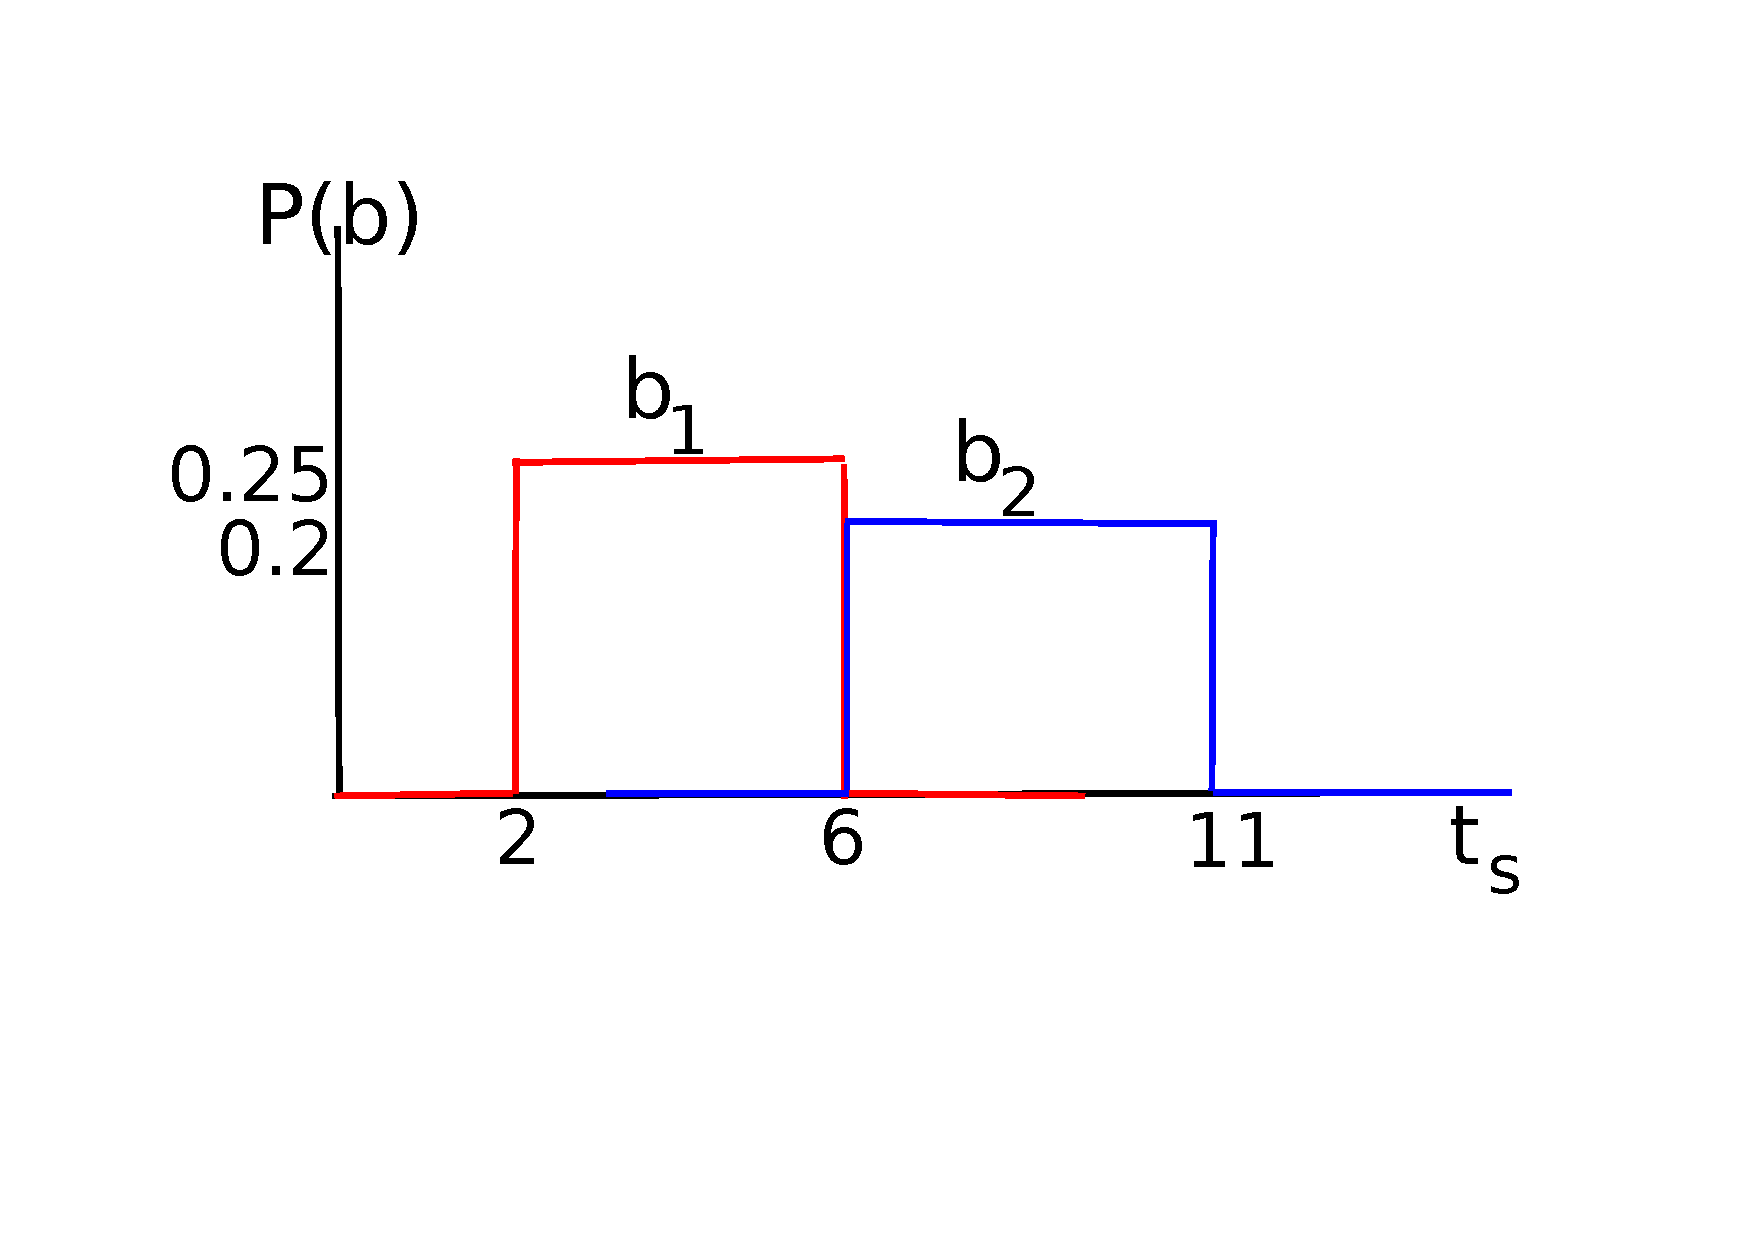
\includegraphics[height=40mm]{pics/beliefs.pdf}
\hspace{-10mm}
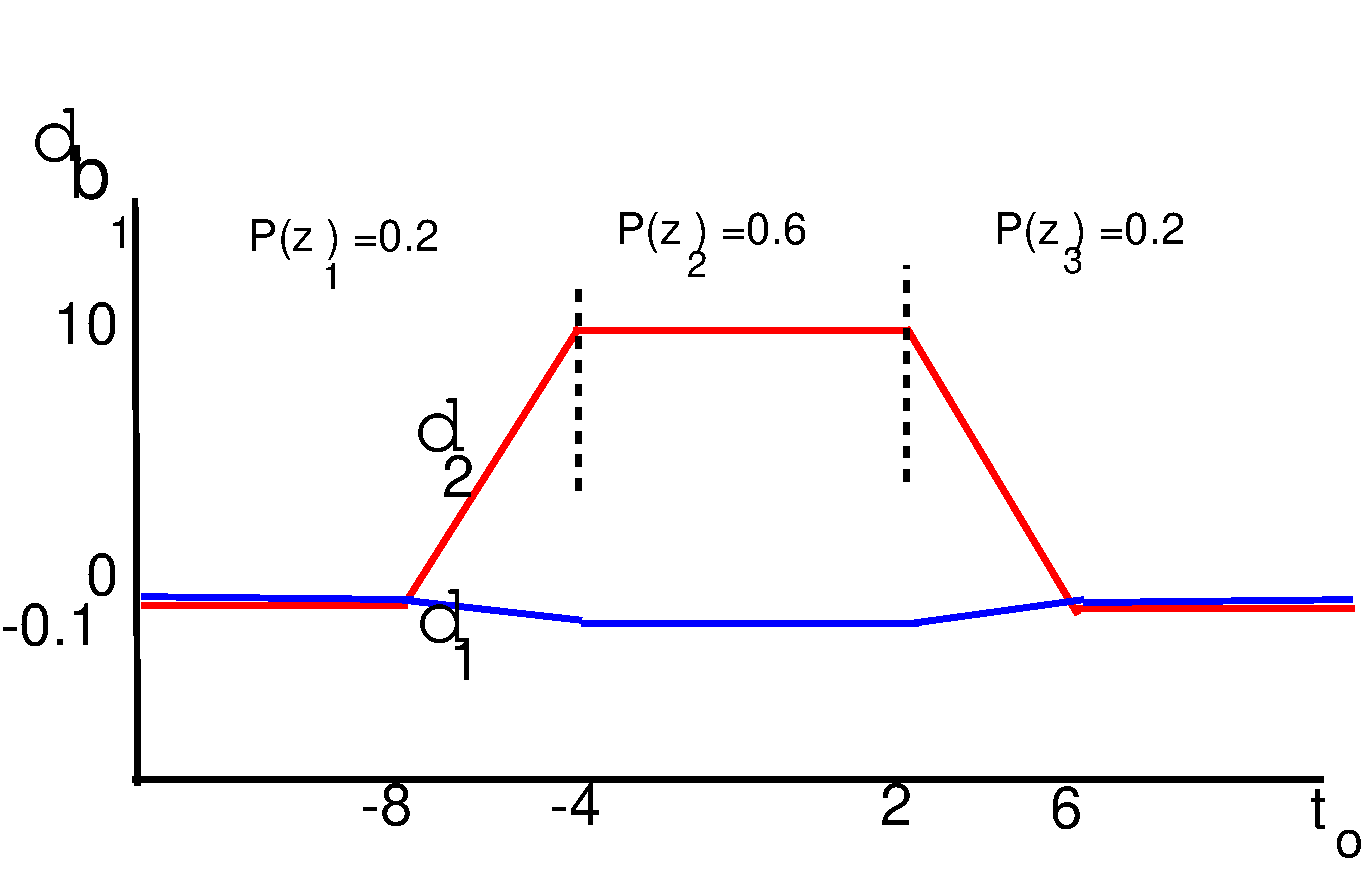
\includegraphics[width=0.33\textwidth]{pics/delta_b1.pdf}
\hspace{-2mm}
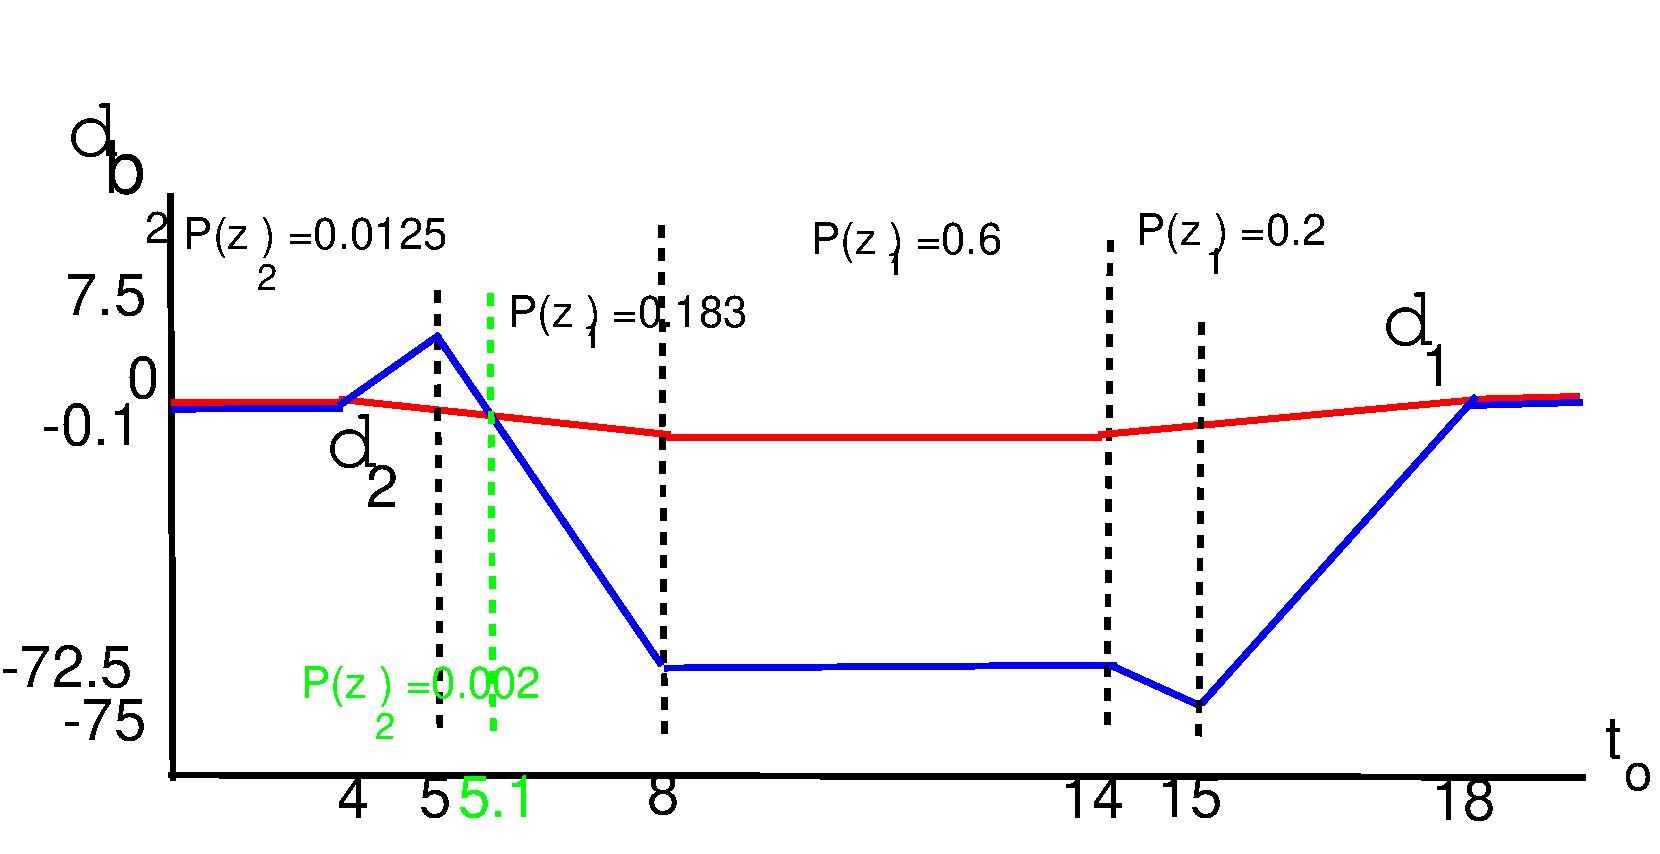
\includegraphics[width=0.42\textwidth]{pics/delta_b2.pdf}
\hspace{-17mm}
\vspace{-2mm}
\caption{\footnotesize 
{\it (left)} Beliefs $b_1,b_2$ for 1D \textsc{\bf Power Plant} example; 
{\it (center)} Observation dependent function for $b_2$ that partition the observation space into 5 regions with different probabilities for $P(z_1),P(z_2)$ ; 
{\it (right)} 3 Relevant observation partitions (which is only one partition) and their probabilities for $b_2$.
}
\label{fig:beliefs}
%\vspace{-4mm}
\end{figure*}
%%%%%%%%%%%%%%%%%%%%%%%%%%%%%%%%%%%%%%%%%%%%%%%%%%%%%%%%%%%%%%%%%%%%%%%%%% 
The observation dependent $\delta$-functions divide the observation space into regions which can yield the optimal policy according to the belief state $b_1$. According to continuous observation space defined in \cite{pascal_ijcai05}, for a 1-dimensional observation space with two or more functions of the observation, we need to find the optimal boundaries or partitions of the space. In their work, numerical solutions are proposed to find the roots of any two observation dependent function. Instead, here we leverage the symbolic power of the max-operator defined in Section~\ref{sec:case} to find all the boundary regions that define for what partitionings of the observation each 
$\delta$-function is optimal. For the two $\delta$-functions above the following partitions of the observation space is derived after taking their maximum in lines 9--11: 
{\footnotesize
\vspace{-2mm}
\begin{align}
\mathrm{max} \Bigg(\delta_{1}(t_o),\delta_{2}(t_o)\Bigg) &= 
\begin{cases}
z_1: (14 < t_o< 18) &: 0.025*t_o - 0.45\\
z_1: (8 < t_o< 14) &:  -0.1\\
z_1: (5.1 < t_o< 8) &: - 0.025*t_o -0.1\\
z_2: (5 < t_o< 5.1) &: - 25*t_o + 127.5\\
z_2: (4 < t_o< 5) &:  2.5*t_o - 10\\
\end{cases}
\nonumber
\end{align}
}
Note here that each partitioned is labeled according to the original $\delta$-function where $z_1$ is the label of the partition coming from $\delta_{1}(t_o)$. 
These partitions define observation regions which we can now use in a similar fashion to a discrete observation set if only the probability of each of the two distinct observation partitions is found.  This is demonstrated visually
in Figure~\ref{fig:beliefs} (center) for $b_2$ and for $b_1$
in Figure~\ref{fig:beliefs} (right). Note here that the maximum of the $\delta$-functions for $b_1$ is equal to $\delta_{2}(t_o)$.

Now with the observation partitions derived, all that remains is to
calculate probabilities for these relevant observations conditioned on
the belief state. 
% This does not check out!
% 
%As a reality check, we note that if we integrate out the
%state and observation from the observation model and the belief state
%regardless of a particular $\alpha$-vector, it integrates to one:
%$\int_{xd_o}\int_{xd_s} P(xd_o|xd'_s,a)*P(xd'_s|xd_s,a)*P(s) = 1$.
Thus we only need to multiply the indicators of each observation partition 
in this formula to obtain the probability mass lying in each
partition:
$$P(z_k|b_i) := \int_{xd_s'}\int_{xd_o}\int_{xd_s} P(xd_o|xd'_s,a)*P(xd'_s|xd_s,a)*b_i* \mathbb{I}[\phi_{z_k}] d_{xd_o} d_{xd_s}d_{xd_s'}$$
For our example the probabilities can be calculated as below:
{\footnotesize
\vspace{-2mm}
\begin{align}
\mathrm{max} \Bigg(\delta_{1}(t_o),\delta_{2}(t_o)\Bigg) &= 
\begin{cases}
(\phi_1 : 14 < t_o< 18) &: 0.2\\
(\phi_2 : 8 < t_o< 14) &:  0.6\\
(\phi_3 : 5.1 < t_o< 8) &: 0.183\\
(\phi_4 : 5 < t_o< 5.1) &: 0.002\\
(\phi_5 : 4 < t_o< 5) &:  0.0125\\
\end{cases}
\nonumber
\end{align}
}
where each constraint is defined as $\phi_i$. For any number of actions and observations the total number of observation partitions depends on the number of belief points. In our example we must have two observation probabilities which is defined as the sum of the probabilities for $z_1,z_2$ according to the constraints: \\
\begin{align*}
z_1&: \phi_1 \vee \phi_2 \vee \phi_3 \longrightarrow P(z_1|b_2)=0.983 \\
z_2&: \phi_4 \vee \phi_5  \longrightarrow P(z_2|b_2)=0.0127
\end{align*}

%{\footnotesize
%\begin{align}
%P(z_k)=
%\begin{cases}
% (t_o<2) &: 0.2 \\
%(2<t_o) &: 0.8\\
%\end{cases} 
%\nonumber
%\end{align}
%}

Hence we can now use the algorithms and methods of a discrete observation setting using the probabilities of the partitioned observation space in PBVI! 
We note here that our method applies to a restricted class of piecewise functions which is piecewise linear transitions and piecewise constant reward and belief. The main reason is that the integration operation over continuous states and observations only allows constant or linear constraints (upper or lower bounds) over these variables \cite{sanner_aaai12}. Thus although in theory we can apply this approach to any piecewise polynomial function, in practice it is limited by the integration bounds.  %Figure ~\ref{fig:obsPartition} shows the observation partitions obtained in the 1D problem instance for different horizons and their related probabilities. In a lyx file, needed?
Next we present some results for 2-dimensional continuous observation spaces.

%%%%%%%%%%%%%%%%%%%%%%%%%%%%%%%%%%%%%%%%%%%%%%%%%%%%%%%%%%%%%%%%%%%%%%%%%%
%\begin{figure}[tbp!]
%\vspace{-2mm}
%\centering
%\includegraphics[width=0.42\textwidth]{pics/nodes.pdf}\\
%\vspace{-2mm}
%\includegraphics[width=0.42\textwidth]{pics/time.pdf}
%\vspace{-2mm}
%\caption{\footnotesize space 
%and time vs. horizon.
%}
%\label{fig:timeSpace}
%\vspace{-4mm}
%\end{figure}
%%%%%%%%%%%%%%%%%%%%%%%%%%%%%%%%%%%%%%%%%%%%%%%%%%%%%%%%%%%%%%%%%%%%%%%%%%

\section{Empirical Results}
We evaluated our continuous POMDP solution using XADDs on the
\textsc{\bf 1D-Power Plant} example and another variant of this
problem with two variables, described below.\footnote{ Full problem
specifications and Java code to reproduce these experiments are available online in
Google Code: \textit{http://code.google.com/p/cpomdp} .}

%%%%%%%%%%%%%%%%%%%%%%%%%%%%%%%%%%%%%%%%%%%%%%%%%%%%%%%%%%%%%%%%%%%%%%%%%%
\begin{figure*}[tbp!]
\vspace{2mm}
\centering
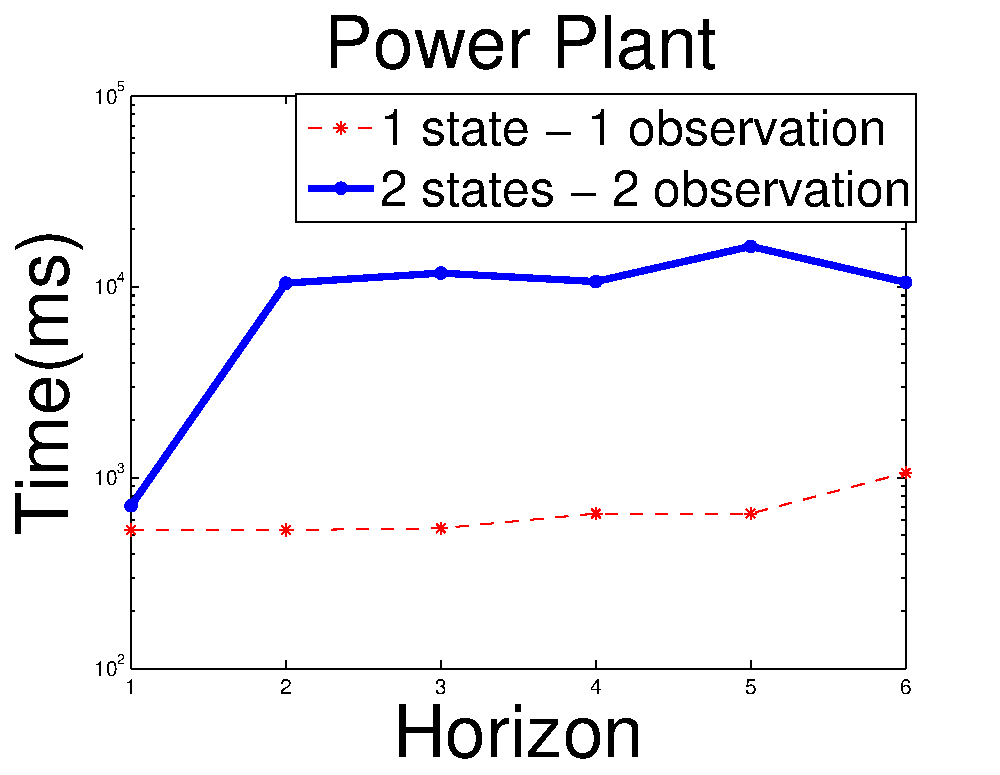
\includegraphics[width=0.32\textwidth]{pics/time2.pdf}
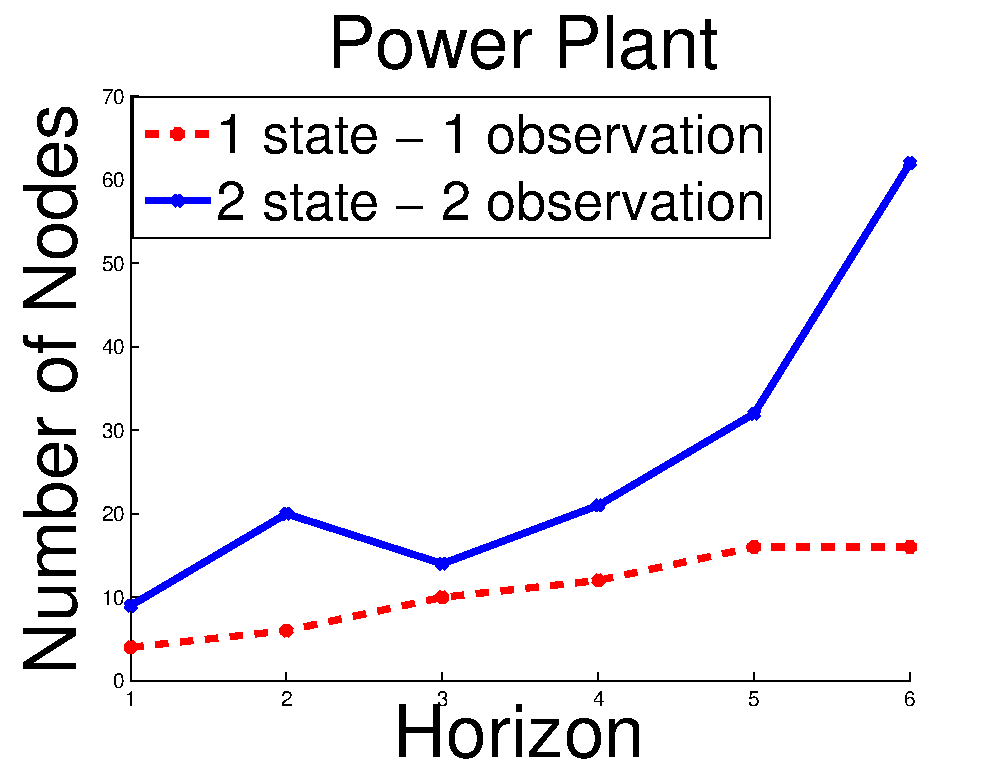
\includegraphics[width=0.32\textwidth]{pics/nodes2.pdf}
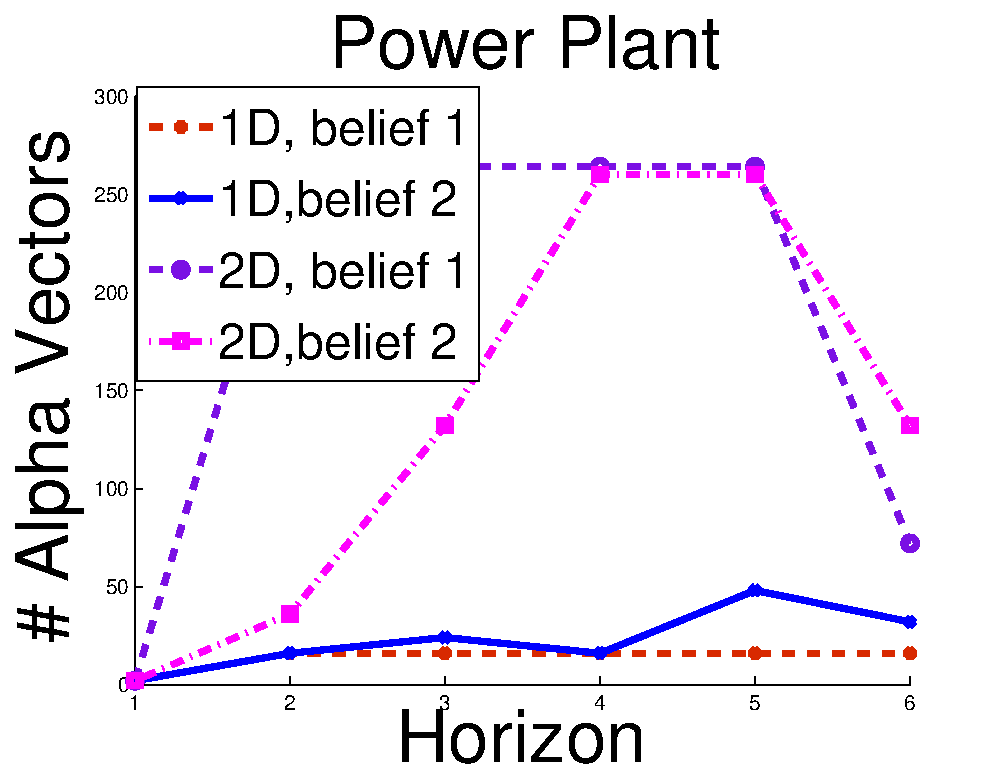
\includegraphics[width=0.32\textwidth]{pics/alpha-vectors2.pdf}
\vspace{-1mm}
\caption{\footnotesize 
{\it (left)} Space vs Horizon; 
{\it (center)} Time vs Horizon; 
{\it (right)} Number of $\alpha$-vectors vs Horizon.
}
\label{fig:timeSpace}
%\vspace{-4mm}
\end{figure*}
%%%%%%%%%%%%%%%%%%%%%%%%%%%%%%%%%%%%%%%%%%%%%%%%%%%%%%%%%%%%%%%%%%%%%%%%%% 

{\bf \textsc{\bf 2D-Power Plant}:} We consider the more complex model of the power plant similar to \cite{steam2} where the pressure inside the water tank must be controlled to avoid mixing water into the steam or explosion of the tank. We model the pressure variable $p$ as a partially observable variable from the observation readings of the pressure $po$. The two actions of increase and decrease are defined based on the change in both the temperature and the pressure. For the increase action we define: %the transition functions and the reward function is defined as below: 
{\footnotesize
\begin{align}
P(p_s'|\vec{p_s},inc)&= \delta\left[ p_s' - 
\begin{cases}
 (p+10> 20) &: 20 \\ 
\neg (p+10> 20) &: p_s + 10 \\
\end{cases}
\right]\nonumber
\hspace{5mm} 
P(t_s'|\vec{t_s},inc)= \delta\left[ t_s' - (t_s +10) \right]\nonumber
\end{align}
}
There is a high reward for staying withing the safe temperature and pressure range since it produces power, else depending on how safe it is to have values higher or lower than the safe range, penalty is defined.
{\footnotesize
\vspace{-3mm}
\begin{align}
R(t_s,p_s,inc) &= 
\begin{cases}
(5 \leq p_s \leq 15)\wedge (95 \leq t_s \leq 105)&:50\\
(5 \leq p_s \leq 15)\wedge (t_s \leq 95)&: -1\\
%(5 \leq p_s \leq 15)\wedge (t_s \geq 95)&: -3\\				
%(p_s \leq 5) &: -3\\						
(p_s \geq 15) &: -5\\ 
else &: -3
\end{cases}\nonumber
\end{align}
}
As for the decrease action, the transition functions reduce the temperature by 5 units and the pressure by 10 units as long as the pressure stays above zero. For the reward function, we assume that there is always a small penalty for decreasing the values because power can not be generated. 
For the observation model we consider two continuous uniform distributions such as the following:  
{\footnotesize
\begin{align}
P(t_o|t_s') = 
\begin{cases}
(t_s + 80<t_o<t_s+ 105) &: 0.4 \\
 \neg (t_s + 80<t_o<t_s+ 105) &: 0 \\
\end{cases}\nonumber
\hspace{5mm} 
P(p_o|p_s') = 
\begin{cases}
(p_s<p_o<p_s+10) &: 0.1 \\
 \neg(p_s<p_o<p_s+10) &: 0 \\
\end{cases}\nonumber
\end{align}
}
We define two rectangular uniform beliefs around the regions of rewarding, so that one needs to increase the values while the other should decrease them: $b_1: U[t_s;90,100]*U[p_s;0,10]$ and $b_2: U[t_s;90,130]*U[p_s;10,30]$
%\begin{align}
%b_1 = 
%\begin{cases}
%(p_o>p_s) \wedge (p_o<p_s+10) \wedge (t_o>t_s+ 90) \wedge (t_o<t_s+ 100)&: 0.01 \\
% \neg( (p_o>p_s) \wedge (p_o<p_s+10) \wedge (t_o>t_s+ 90) \wedge (t_o<t_s+ 100)) &: 0 \\
%\end{cases}\nonumber
%\end{align}
%\begin{align}
%b_2 = 
%\begin{cases}
%(p_o>p_s +10) \wedge (p_o<p_s+30) \wedge (t_o>t_s+ 90) \wedge (t_o<t_s+ 130)&: 0.00125 \\
% \neg((p_o>p_s +10) \wedge (p_o<p_s+30) \wedge (t_o>t_s+ 90) \wedge (t_o<t_s+ 130)) &: 0 
%\end{cases}\nonumber
%\end{align}
% I can draw this and the 1D belief
In Figure ~\ref{fig:timeSpace}, a time and space analysis of
the two versions of \textsc{\bf Power Plant} have been performed for up to 6 horizons. %Comparing the two problem sizes demonstrates the effect of the number of state-observation variables in our algorithm. 
As the algorithm progresses, the time required to compute the probability of the partitions and finding the maximum $\alpha$-vector with respect to beliefs increases for both problem sizes and significantly more for the 2D version. %The stability in time is due to the fact that each stage almost takes the same time since it has converged quickly.%???
Increase in the problem size, increases the partition numbers on the observation space and this produces more $\alpha$-vectors which also effects the space required to perform the algorithm. The number of vectors stays the same for most horizons and they drop after convergence in the 2D problem instance. %The number of nodes in each iteration increases as more space is required to perform higher iterations.
This shows that although the 2D instance takes more time and space than the 1D instance, it still converges within reasonable resources.

In Figure ~\ref{fig:3D}  we present plots of the maximum $\alpha$-vectors of belief $b_1$ for different iterations of the 2D problem instance. %Each plot demonstrates the value of each vector as a function of the pressure and temperature. 
Starting with the first iteration, the value is highest for the reward range ($5<p<15 \wedge 95<t<105$) and -1 or less for other places. In the fifth iteration, the value function has partitioned into more pieces, showing how higher temperatures can increase the value without considering the effect of the pressure. In the last plot, horizon $h=6$ has better tuned the value function so that higher temperatures and pressures increase the value of the maximum $\alpha$-vector and also within the reward range, finer grain partitions have been formed. %Also note that the policy depends on the initial belief and for these plots they were based on $b_1$ which was lower than the reward range. The first action would then mean it has performed an increase while the other iterations decrease and increase respectively.  
%%%%%%%%%%%%%%%%%%%%%%%%%%%%%%%%%%%%%%%%%%%%%%%%%%%%%%%%%%%%%%%%%%%%%%%%%%
% policy2, v2plot.pdf, v9plot
% annotation?
\begin{figure*}[tbp!]
%\vspace{-2mm}
\centering
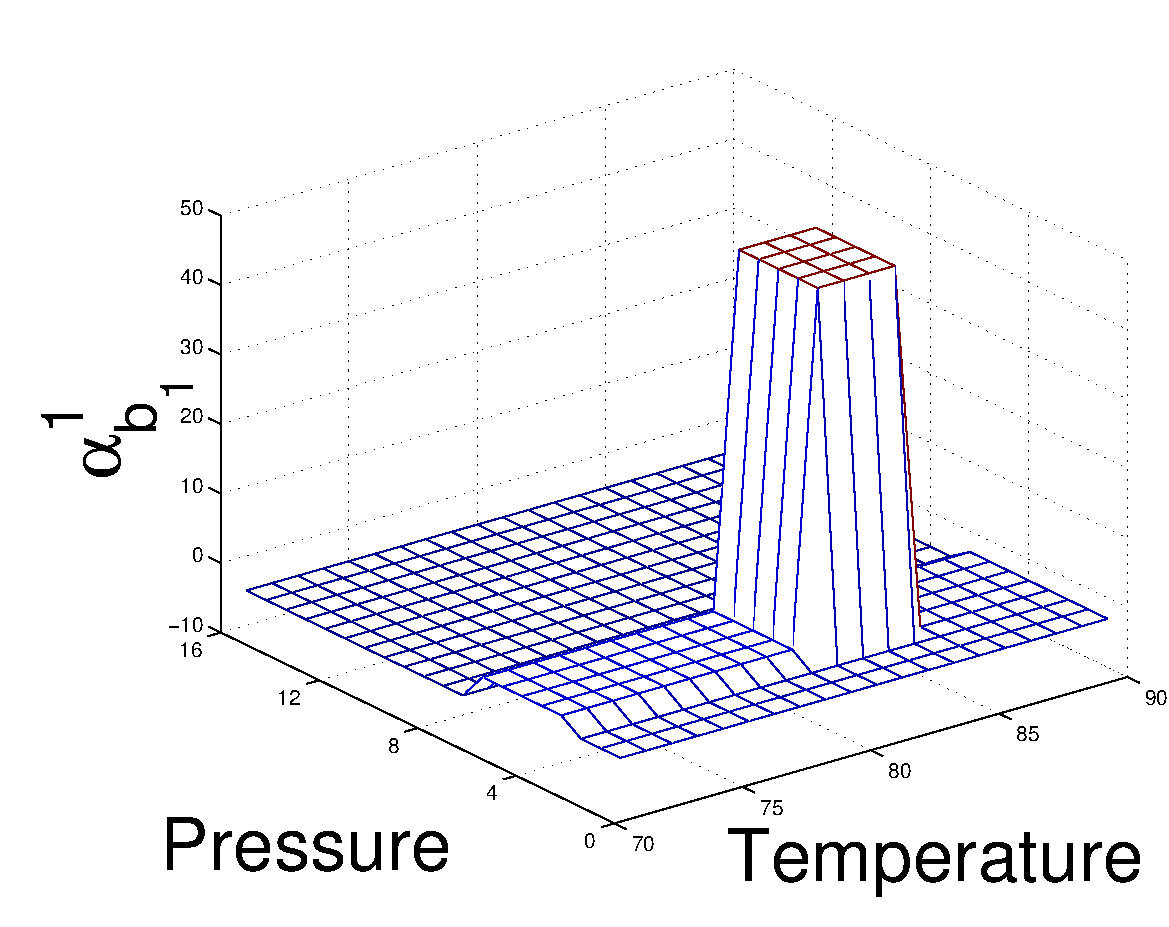
\includegraphics[width=0.31\textwidth]{pics/2d1.pdf}
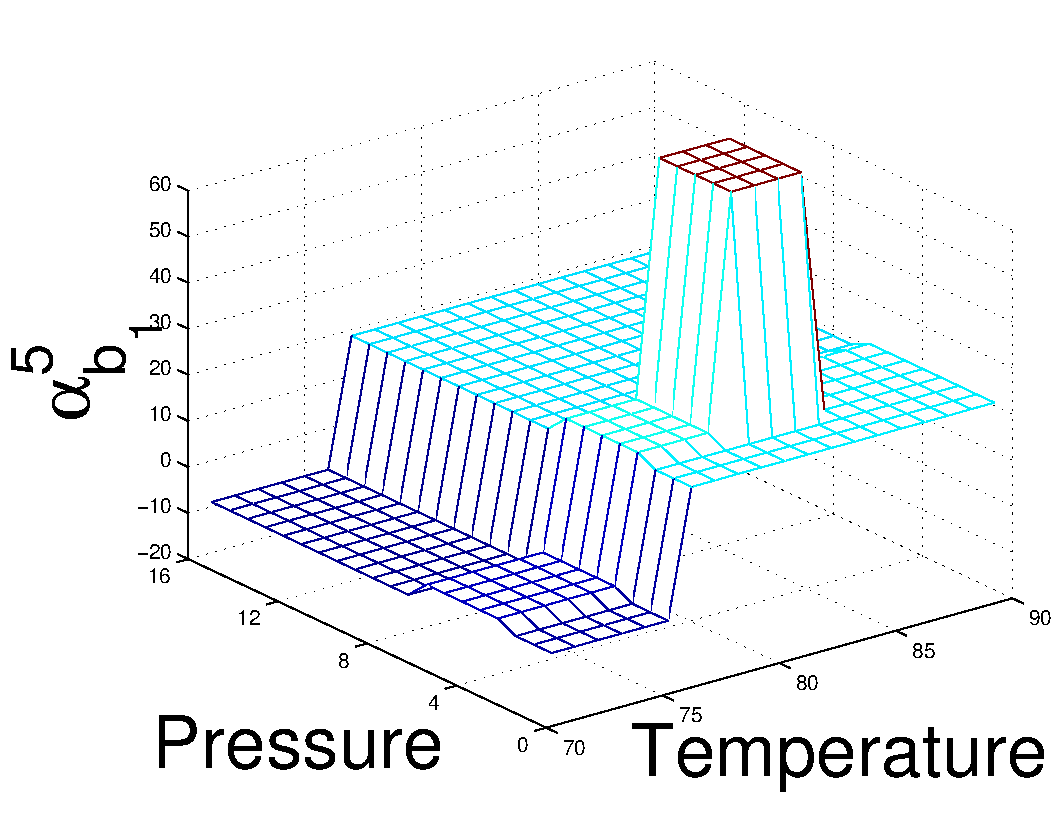
\includegraphics[width=0.31\textwidth]{pics/2d9.pdf}
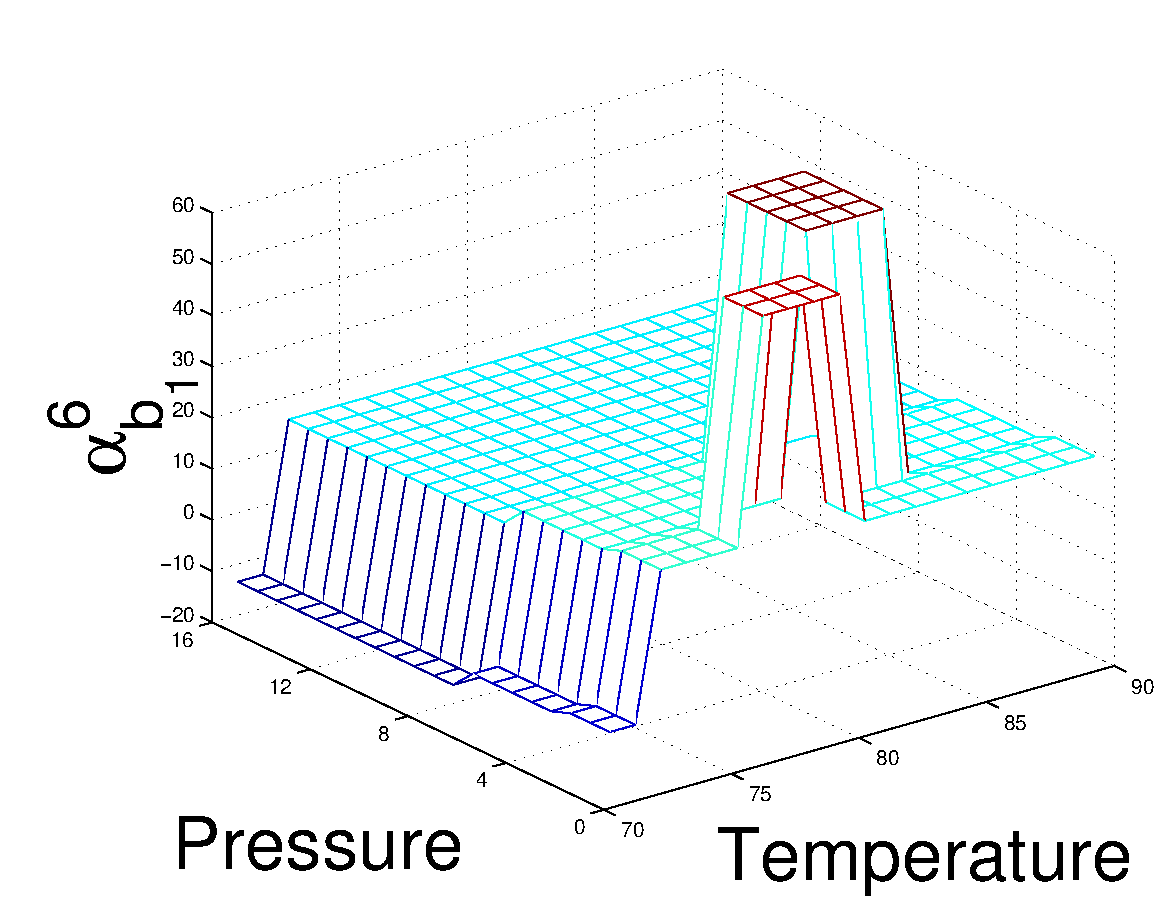
\includegraphics[width=0.31\textwidth]{pics/2d111.pdf}
\vspace{-3mm}
\caption{\footnotesize 
{\it (left)}Maximum $\alpha$-vector for $b_1$ in first iteration; 
{\it (center)} $\alpha_{max}^5(b_1)$; 
{\it (right)} $\alpha_{max}^5(b_1)$.%V^6(p,t)
}
\label{fig:3D}
%\vspace{-4mm}
\end{figure*}
%%%%%%%%%%%%%%%%%%%%%%%%%%%%%%%%%%%%%%%%%%%%%%%%%%%%%%%%%%%%%%%%%%%%%%%%%% 

\section{Conclusion} 
%This work has used the concept of continuous states and the SDP solution to MDPs from ~\cite{sanner_uai11} and continuous observations from the work of \cite{pascal_ijcai05}. It is exclusive in the sense that it brings together the continuous state and observation POMDPs using a symbolic approach. 
%In many applications of the POMDP framework, the state and observation space have been considered as discrete values such as ~\cite{steam2} here we avoid this general simplification and work with the real values from sensors.
%%sampling, monte carlo, particle filter, gaussians, perseus, pergeus
%
%There has been prior work on approximate solutions to POMDPs with large or continuous state spaces ~\cite{Thrun99h}, ~\cite{Perseus} and some has been extended to the continuous observation setting using methods such as sampling ~\cite{Perseus_cont}.
%In most approximate continuous state POMDP work, continuous or large discrete actions has been used. Thus we can extend the current work using \cite{zamani_aaai12} to contain continuous actions and provide exact or approximate solutions. 
%
%%\section{Conclusion}
We presented the first exact symbolic operations for \texttt{PBVI} in
expressive DC-POMDPs with continuous state \emph{and} observations.
Unlike related work that has extended to the continuous state and
observation setting~\cite{Perseus_cont}, we do not approach the
problem by sampling.  Rather, following~\cite{pascal_ijcai05}, the key
contribution of this work was to define a discrete set of observation
partitions on the multivariate continuous observation space via
symbolic maximization techniques and derive the related probabilities
using symbolic integration.  An important avenue for future work is to
determine whether similar techniques can be applied to the difficult
case of continuous state, observation, \emph{and} action DC-POMDPs.

%\subsubsection*{References} 
\bibliography{dcpomdp}
\bibliographystyle{plain}

\end{document}